\newpage
\section{Results}

\subsection{Virtual constraints controller}

When optimizing on the objective function~\ref{eq::virtual_constraints_objective_fun} with $w_1 = w_2 = 0.5$, and $\dot{x} = \SI{0.7}{\meter\per\second}$, the following set of optimized parameters were computed:

\begin{align*}
	\mathbf{q}_0 &= \begin{bmatrix}
		0.3239 \\ -0.3496 \\ \num{3.746e-4}
	\end{bmatrix} \\
	\mathbf{\dot{q}}_0 &= \begin{bmatrix}
		\num{2.894e-04} \\ \num{1.720e-04} \\ 8.583
	\end{bmatrix} \\
	k_{p1} &= 452.6 \\
	k_{p2} &= 102.1 \\
	k_{d1} &= 95.15 \\
	k_{d2} &= 4.619 \\
	\alpha &= 0.1911
\end{align*}

The state-space plot displayed on Figure~\ref{img::virtual_constraints_state_space} are a great way to assess whether the gait is stable, and after how long.
Indeed, on Figure~\ref{img::virtual_constraints_state_space}, we can observe that the first two steps are not in a steady-state yet.
Only starting from step three and onward (out of ten steps) is the gait stable, and that is illustrated by the state-space plots looping back on themselves.
Even like so, the third step is not quite steady for the top link of the robot before the fourth step.


\begin{figure}[H]
	\begin{subfigure}[h]{0.35\textwidth}
		\begin{center}
			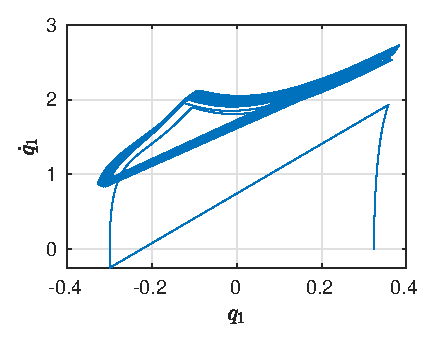
\includegraphics[width=\textwidth]{a04_state_space_q1_optimized}
			\caption{$q_1$ state-space plot}
		\end{center}
	\end{subfigure}
	\begin{subfigure}[h]{0.35\textwidth}
		\begin{center}
			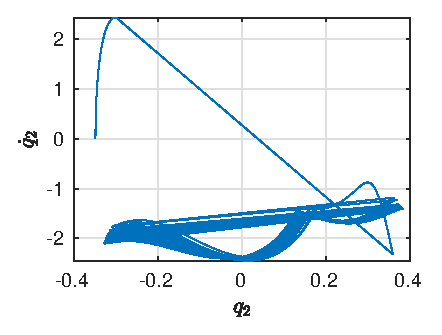
\includegraphics[width=\textwidth]{a04_state_space_q2_optimized}
			\caption{$q_2$ state-space plot}
		\end{center}
	\end{subfigure}
	
	\begin{subfigure}[h]{0.35\textwidth}
		\begin{center}
			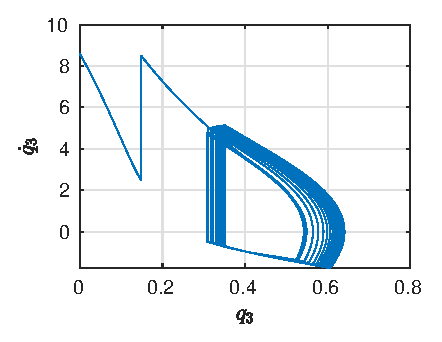
\includegraphics[width=\textwidth]{a04_state_space_q3_optimized}
			\caption{$q_3$ state-space plot}
		\end{center}
	\end{subfigure}
	\caption{State-space plot for the three generalized coordinates.}
	\label{img::virtual_constraints_state_space}
\end{figure}

Then, when looking at the position of the hip along time on Figure~\ref{fig::virtual_constraints_hip_position}, we can make a few observations:

\begin{itemize}
	\item the stability of the gait as assessed from the state-space plots is confirmed by those plots: the first two steps are not in steady-state, but the subsequent steps have a periodic aspect,
	\item vertically, the hip oscillates,
	\item while horizontally, it's advancing at a constant rate.
\end{itemize}


\begin{figure}[H]
	\begin{subfigure}[h]{0.6\textwidth}
		\begin{center}
			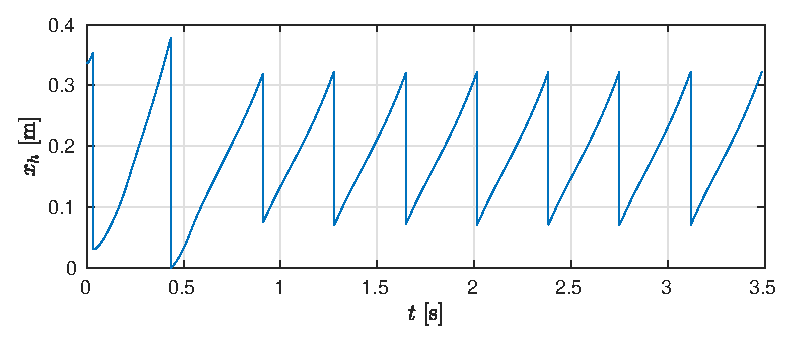
\includegraphics[width=\textwidth]{a04_x_h}
			\caption{horizontal position of the hip}
		\end{center}
	\end{subfigure}
	\begin{subfigure}[h]{0.6\textwidth}
		\begin{center}
			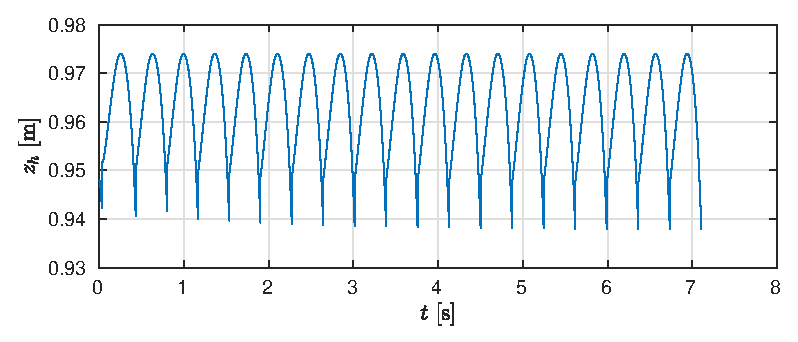
\includegraphics[width=\textwidth]{a04_z_h}
			\caption{vertical position of the hip}
		\end{center}
	\end{subfigure}
	\caption{Position of the hip as a function of time.}
	\label{fig::virtual_constraints_hip_position}
\end{figure}

The saturation of the command is effective on $u_1$, but $u_2$ doesn't reach the maximum, so the saturation doesn't have an effect on it, as can be seen on Figure~\ref{fig::virtual_constraints_commands}:

\begin{figure}[H]
	\begin{subfigure}[h]{0.35\textwidth}
		\begin{center}
			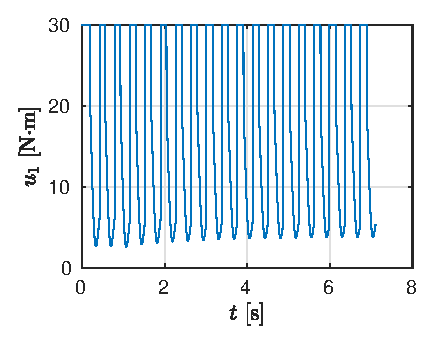
\includegraphics[width=\textwidth]{a04_control_torques_u1_optimized}
			\caption{first actuator}
		\end{center}
	\end{subfigure}
	\begin{subfigure}[h]{0.35\textwidth}
		\begin{center}
			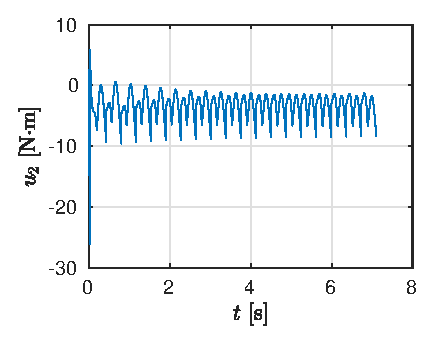
\includegraphics[width=\textwidth]{a04_control_torques_u2_optimized}
			\caption{second actuator}
		\end{center}
	\end{subfigure}
	\caption{Command angles in function of time for both actuators.}
	\label{fig::virtual_constraints_commands}
\end{figure}

Also, the horizontal velocity of the hip stabilizes after the third step, and in the steady-state, oscillates between \SI{0.6}{\meter\per\second} and \SI{0.9}{\meter\per\second}, as can be seen on Figure~\ref{fig::virtual_constraints_hip_velocity} (left).
In particular, when looking at the velocity averaged on each step on Figure~\ref{fig::virtual_constraints_hip_velocity} (right), it reaches at steady-state the average velocity of $\sim\SI{0.74}{\meter\per\second}$ for a target of \SI{0.7}{\meter\per\second}:

\begin{figure}[H]
	\begin{subfigure}[h]{0.35\textwidth}
		\begin{center}
			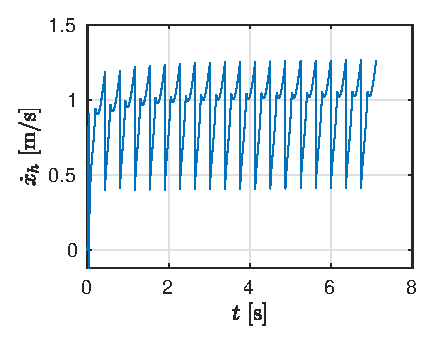
\includegraphics[width=\textwidth]{a04_dx_h}
			\caption{velocity of the hip}
		\end{center}
	\end{subfigure}
	\begin{subfigure}[h]{0.35\textwidth}
		\begin{center}
			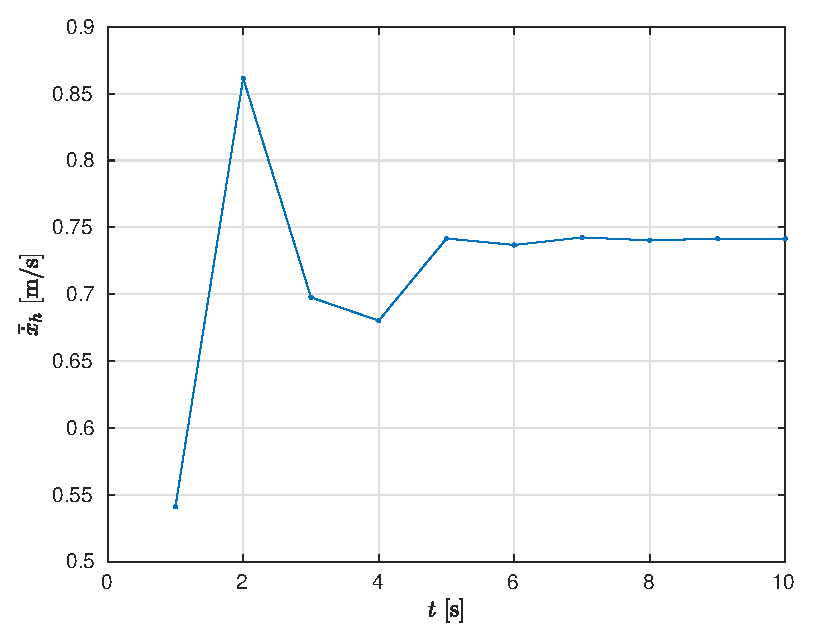
\includegraphics[width=\textwidth]{a04_average_dx_h}
			\caption{velocity of the hip averaged over the steps}
		\end{center}
	\end{subfigure}
	\caption{Velocity  of the hip in function of time / steps.}
	\label{fig::virtual_constraints_hip_velocity}
\end{figure}

The plots of the step frequencies and durations (Figure~\ref{fig::virtual_constraints_step_regularity}) allow to assess, once again, that after the third step, the robot is in steady-state, because the frequency of the step stabilizes afterwards.

\begin{figure}[H]
	\begin{subfigure}[h]{0.35\textwidth}
		\begin{center}
			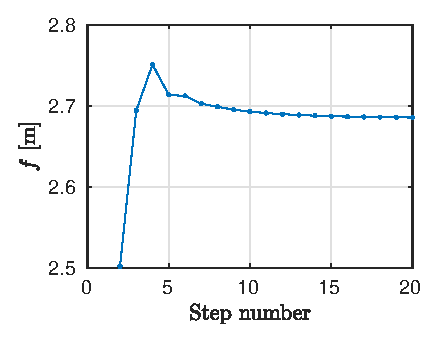
\includegraphics[width=\textwidth]{a04_step_frequency}
			\caption{step frequency}
		\end{center}
	\end{subfigure}
	\begin{subfigure}[h]{0.35\textwidth}
		\begin{center}
			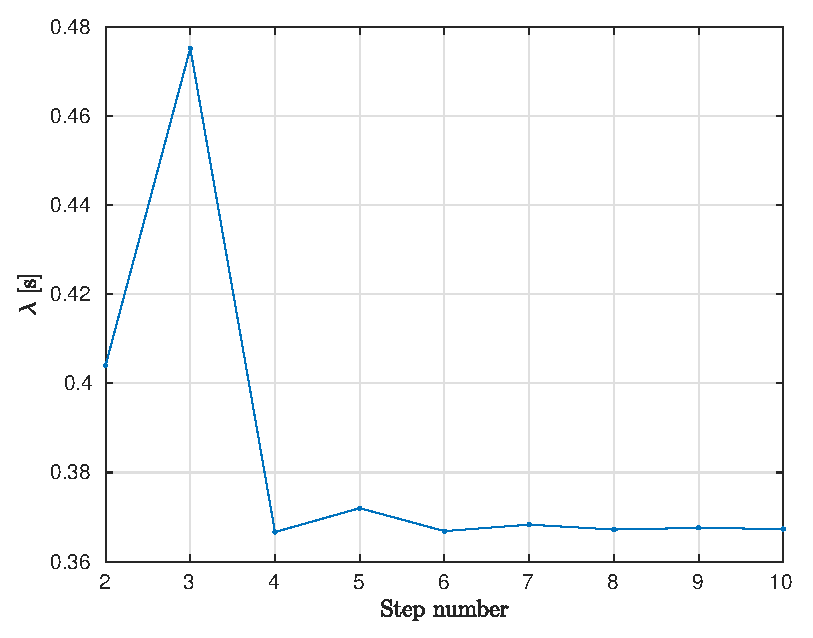
\includegraphics[width=\textwidth]{a04_step_lambda}
			\caption{step duration}
		\end{center}
	\end{subfigure}
	\caption{Regularity of the stepping.}
	\label{fig::virtual_constraints_step_regularity}
\end{figure}

The normalized mean effort is \SI{4.23}{\newton\meter\per\second}, and the CMT is \num{6.524e-3}.

\subsection{Virtual model controller}

When optimizing on the objective function~\ref{eq::virtual_model_objective_fun} with:

\begin{itemize}
	\item $w_1 = 1$,
	\item $w_2 = 10$,
	\item $w_3=200$,
	\item $w_4=-1$,
	\item $w_5=20$,
	\item $\dot{x} = \SI{0.7}{\meter\per\second}$,
	\item $z_\text{hip d} = \SI{0.35}{\meter}$,
	\item and $f_\text{d} = \SI{2.5}{\hertz}$.
\end{itemize}

On Figure~\ref{img::virtual_model_state_space}, we can observe that the steady-state is reached faster than with the virtual constraints controller, namely, at the second step already.

\begin{figure}[H]
	\begin{subfigure}[h]{0.35\textwidth}
		\begin{center}
			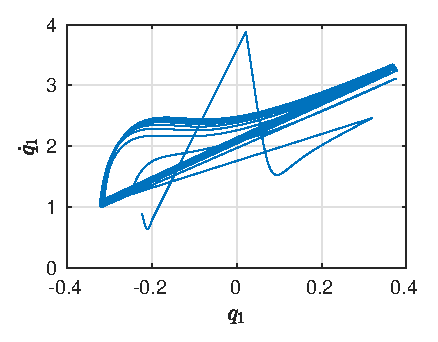
\includegraphics[width=\textwidth]{a05_state_space_q1_optimized}
			\caption{$q_1$ state-space plot}
		\end{center}
	\end{subfigure}
	\begin{subfigure}[h]{0.35\textwidth}
		\begin{center}
			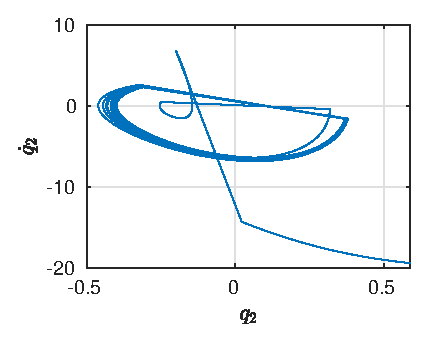
\includegraphics[width=\textwidth]{a05_state_space_q2_optimized}
			\caption{$q_2$ state-space plot}
		\end{center}
	\end{subfigure}
	
	\begin{subfigure}[h]{0.35\textwidth}
		\begin{center}
			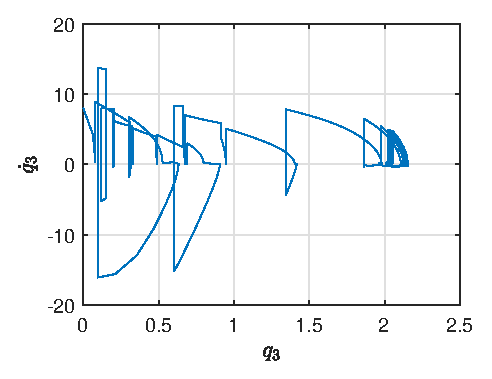
\includegraphics[width=\textwidth]{a05_state_space_q3_optimized}
			\caption{$q_3$ state-space plot}
		\end{center}
	\end{subfigure}
	\caption{State-space plot for the three generalized coordinates.}
	\label{img::virtual_model_state_space}
\end{figure}

Then, when looking at the position of the hip along time on Figure~\ref{fig::virtual_model_hip_position}, we can make observations similar to the ones for the virtual constraints controller:

\begin{itemize}
	\item the stability of the gait is reached at the second state, as precedently observed on the state-space plots,
	\item vertically, the hip oscillates,
	\item while horizontally, it's advancing at a constant rate.
\end{itemize}


\begin{figure}[H]
	\begin{subfigure}[h]{0.6\textwidth}
		\begin{center}
			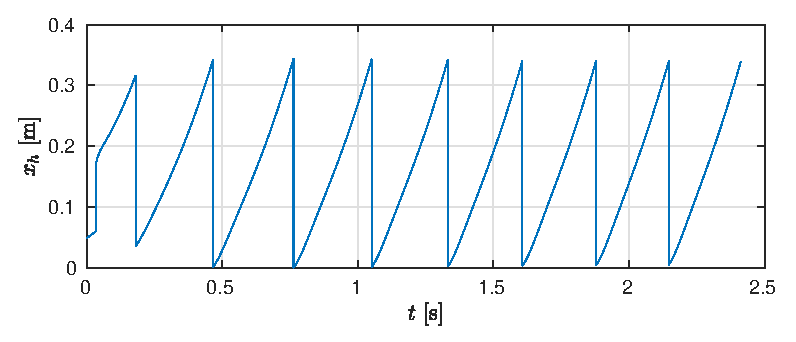
\includegraphics[width=\textwidth]{a05_x_h}
			\caption{horizontal position of the hip}
		\end{center}
	\end{subfigure}
	\begin{subfigure}[h]{0.6\textwidth}
		\begin{center}
			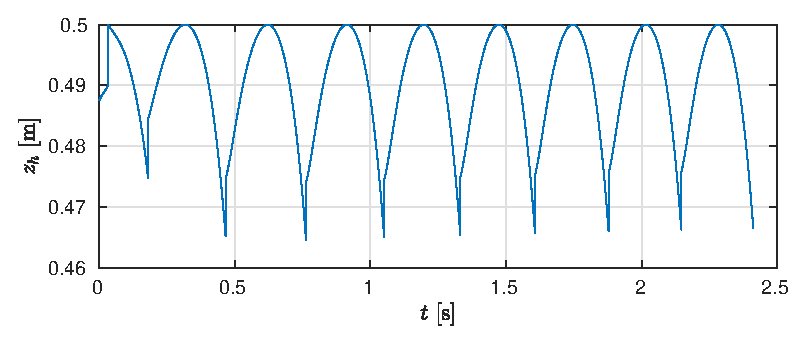
\includegraphics[width=\textwidth]{a05_z_h}
			\caption{vertical position of the hip}
		\end{center}
	\end{subfigure}
	\caption{Position of the hip as a function of time.}
	\label{fig::virtual_model_hip_position}
\end{figure}

None of the commands $\mathbf{u}$ saturate, as can be seen on Figure~\ref{fig::virtual_model_commands}:


\begin{figure}[H]
	\begin{subfigure}[h]{0.35\textwidth}
		\begin{center}
			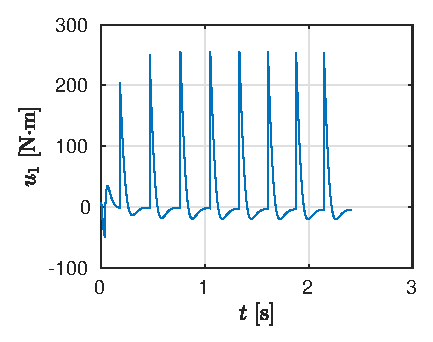
\includegraphics[width=\textwidth]{a05_control_torques_u1_optimized}
			\caption{first actuator}
		\end{center}
	\end{subfigure}
	\begin{subfigure}[h]{0.35\textwidth}
		\begin{center}
			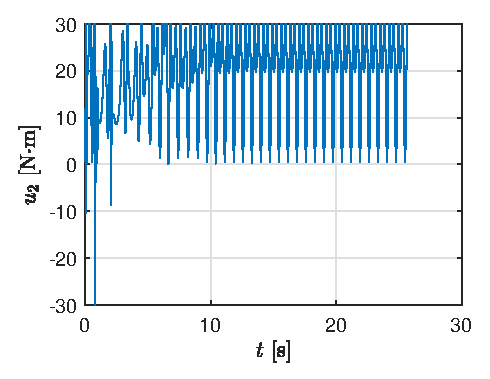
\includegraphics[width=\textwidth]{a05_control_torques_u2_optimized}
			\caption{second actuator}
		\end{center}
	\end{subfigure}
	\caption{Command angles in function of time for both actuators.}
	\label{fig::virtual_model_commands}
\end{figure}

Also, the horizontal velocity of the hip stabilizes after the second step, and in the steady-state, oscillates between \SI{0.5}{\meter\per\second} and \SI{1.5}{\meter\per\second}, as can be seen on Figure~\ref{fig::virtual_model_hip_velocity} (left).
In particular, when looking at the velocity averaged on each step on Figure~\ref{fig::virtual_model_hip_velocity} (right), it reaches at steady-state the average velocity of $\sim\SI{1.1}{\meter\per\second}$ for a target of \SI{0.5}{\meter\per\second}.

\begin{figure}[H]
	\begin{subfigure}[h]{0.35\textwidth}
		\begin{center}
			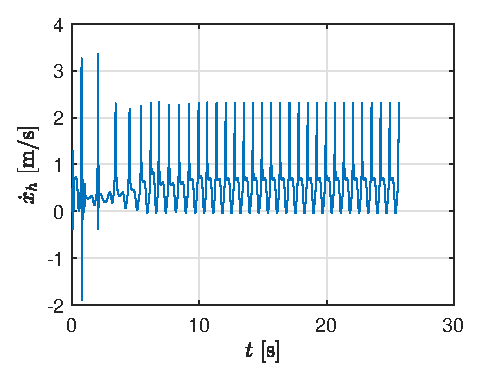
\includegraphics[width=\textwidth]{a05_dx_h}
			\caption{velocity of the hip}
		\end{center}
	\end{subfigure}
	\begin{subfigure}[h]{0.35\textwidth}
		\begin{center}
			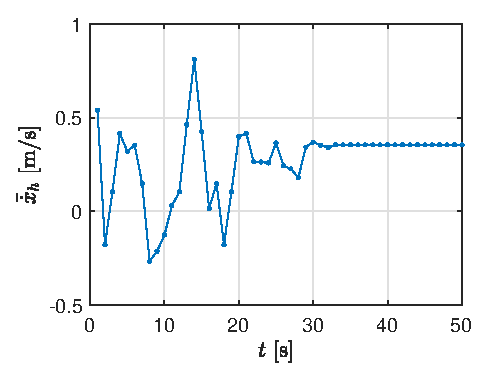
\includegraphics[width=\textwidth]{a05_average_dx_h}
			\caption{velocity of the hip averaged over the steps}
		\end{center}
	\end{subfigure}
	\caption{Velocity  of the hip in function of time / steps.}
	\label{fig::virtual_model_hip_velocity}
\end{figure}

The plots of the step frequencies and durations (Figure~\ref{fig::virtual_model_step_regularity}) allow to assess, once again, that after the second step, the robot is in steady-state, because the frequency of the step stabilizes afterwards.

\begin{figure}[H]
	\begin{subfigure}[h]{0.35\textwidth}
		\begin{center}
			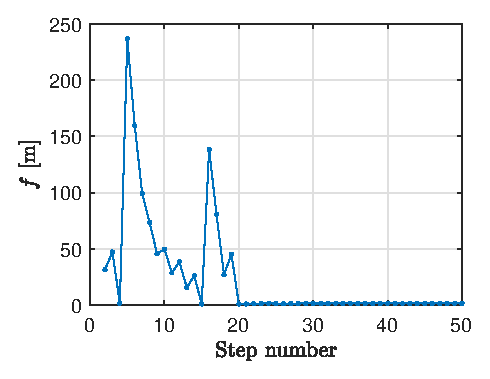
\includegraphics[width=\textwidth]{a05_step_frequency}
			\caption{step frequency}
		\end{center}
	\end{subfigure}
	\begin{subfigure}[h]{0.35\textwidth}
		\begin{center}
			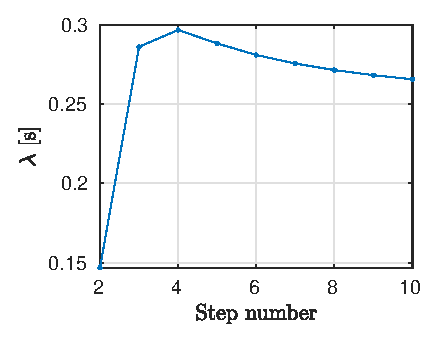
\includegraphics[width=\textwidth]{a05_step_lambda}
			\caption{step duration}
		\end{center}
	\end{subfigure}
	\caption{Regularity of the stepping.}
	\label{fig::virtual_model_step_regularity}
\end{figure}

The normalized mean effort is \SI{80.4321}{\newton\meter\per\second}, and CMT is \num{0.2024}.
